\documentclass {article}

\usepackage{color}
\usepackage{caption}
\usepackage{wrapfig}
\usepackage{graphicx}
\usepackage{amsmath}
\usepackage{amssymb}
\usepackage{mathtools}
\usepackage{amsfonts} % pour les lettres maths creuses \mathbb{•}}
\usepackage{mathrsfs} % pour les lettres maths arrondies \mathscr{•}
\usepackage{algorithm}
\usepackage{algpseudocode}  %\usepackage[noend]{algpseudocode}
\algtext*{EndWhile}% Remove "end while" text
\algtext*{EndIf}% Remove "end if" text
\algdef{SE}[DOWHILE]{Do}{doWhile}{\algorithmicdo}[1]{\algorithmicwhile\ #1}

\title {Gradient-Based Path Optimization}
% Author : Mylene Campana and Florent Lamiraux

\newcommand\p{\mathbf{p_i}}
\newcommand\giT{\tilde{g_i}^T}
\newcommand\gi{\tilde{g_i}}
\newcommand\Jfi{J_{f_i}}
\newcommand\real{\mathbb{R}}
\newcommand\tcollk{t_{coll_k}}

\newcommand\myeq{\stackrel{\mathclap{\normalfont\mbox{desired}}}{=}}


%%%%%%%%%%%%%%%%%%%%%%%%%%%%%%%%%%%%%%%%%%%%%%%%%%%%%%%%%%%%%%%%%%%%%%%%%%%%%%%%
\begin{document}
\maketitle

\tableofcontents

\newpage

%%%%%%%%%%%%%%%%%%%%%%%%%%%%%%%%%%%%%%%%%%%%%%%%%%%%%%%%%%%%%%%%%%%%%%%%%%%%%%%%
\section{Assumptions}

The path optimizer reduces the length of a given path with some assumptions:
\begin{itemize}
\item The cost is defined in a vectorial space (i.e., rotations must be defined by bounded rotations, $SO_3$ joint can not be directly used). This provides a quadratic cost.

\item The cost can be weighted by the proportionality of the initial segments lengths (see weighted cost definition). You can force to one weights in the code to cancel weighting.

\item we do not have convergence proof of solving a quadratic cost under non-linear constraints.

\end{itemize}



\newpage

%%%%%%%%%%%%%%%%%%%%%%%%%%%%%%%%%%%%%%%%%%%%%%%%%%%%%%%%%%%%%%%%%%%%%%%%%%%%%%%%
\section{Collision Constraints}
\subsection{Notations}
$c(x)$ : cost
$x$ : path defined by the waypoints. \\
$\mathbf{p}$ : gradient direction of iteration (obtained with BFGS algorithm 
$p = -H^{-1}\nabla c(x)$). \\
$\alpha$ : tuning parameter. \\
$J_f$ : collision constraints jacobian



\subsection{Constraints}
Affine constraints: \\
Every path apply previous constraints. \\
$x_{2i}$ : paths on which computed constraints are backtracked. \\
$x_{2i+1}$ : paths with high probability of collisions on which $J_f$ is 
computed. \\
Newton algorithm : $ x_{2i+1} = x_{2i} + \alpha_{2i} \mathbf{p_{2i}} $ \\
\\
Constraint definition : $ f(x_{i+2}) = f(x_{i}) $ \\
\begin{eqnarray}
f(x_{i+2}) - f(x_{i+1}) &=& f(x_i) - f(x_{i+1}) \\
\frac{\partial{f(x_{i+1})}}{\partial{x}}(x_{i+2}-x_{i+1}) &=& 
-\frac{\partial{f(x_{i})}}{\partial{x}}(x_{i+1}-x_{i})\\
\Jfi(x_{i+2}-x_{i+1}) &=& \Jfi(x_{i+1}-x_i) \\
\alpha_{i+1} \Jfi \mathbf{p_{i+1}} &=& - \alpha_i \Jfi  \p \ \ \  \\
\end{eqnarray}

Because the constraint (jacobian) is computed only once every two iterations, 
$$\frac{\partial{f(x_{i+1})}}{\partial{x}} = \frac{\partial{f(x_{i})}}
{\partial{x}} = \Jfi$$

So the affine constraint can be globally written as:
$$ \Jfi \mathbf{p} = b $$

with the second term (which is zero for a linear constraint)
$$ b = \frac{\alpha}{\alpha_{previous}} J_{f} \mathbf{p_{previous}}$$

That formula avoids to directly compute the constraint ($f(q_{Constr}) = b$) 
using forward kinematics, all terms are already available.

$ \mathbf{p_{previous}} $ depends how affine constraints are used. Section 
\ref{section:naiveProjectionSection} presents an example of ```compute and apply 
constraint one step over two'', so $ \mathbf{p_{previous}} $ is basically the 
previous performed step.



\subsection{Example of algorithm using naive step projection on affine 
constraints null space} \label{section:naiveProjectionSection}
Projection of $\mathbf{p_{i+1}}$ direction:
$$\mathbf{\overline{p_{i+1}}} = (I-\Jfi^{+}\Jfi) \mathbf{p_{i+1}} - 
\frac{\alpha_i}{\alpha_{i+1}} \Jfi^{+}\Jfi \p$$\\
$x_0$ : paths with no constraint and collision-free. \\
\\
$x_1 = x_0 + \alpha_0 \mathbf{p_0}$ : path with collision $q_{Coll_0}$ and no 
constraint, computes future constraint $q_{Constr_0}$, add it to $J_f$.\\
\\
$x_2$ : path which project the gradient descent $\mathbf{p_1}$ to comply with 
the constraint $q_{Constr_0}$. Works also with several constraints added at the 
same time. \\
$x_2 = x_1 + \alpha_1 \mathbf{\overline{p_1}}$ \\
$\mathbf{\overline{p_1}} = (I-J_f^{+}J_f) \mathbf{p_1} - \frac{\alpha_0}
{\alpha_1}J_f^{+}J_f \mathbf{p_0}$ \\
\\
$x_3$ : path which project the gradient descent $\mathbf{p_2}$ to comply with 
the constraint $q_{Constr_0}$, in collision $q_{Coll_1}$, so create $q_{Constr_1}$ 
and update $J_f$. \\
$x_3 = x_2 + \alpha_2 \mathbf{\overline{p_2}}$ \\
$\mathbf{\overline{p_2}} = (I-J_f^{+}J_f) \mathbf{p_2}$ \\
No affine term since $x_2$ already applied the constraint. \\
\\
$x_4$ : path which project the gradient descent $\mathbf{p_3}$ to comply with 
the constraints $q_{Constr_0}$ and $q_{Constr_1}$. \\
$x_4 = x_3 + \alpha_3 \mathbf{\overline{p_3}}$ \\
$\mathbf{\overline{p_3}} = (I-J_f^{+}J_f) \mathbf{p_3} - \frac{\alpha_2}
{\alpha_3} J_f^{+}J_f \mathbf{p_2}$ \\

Problem encountered : we will get the solution of the constraint sub-space 
that is orthogonal to $-H^{-1}\nabla c(x)$ but it will not minimize the 
quadratic cost. This is why the section \ref{section:lagoLLTSection} is rather solving 
a QP under constraints.

\subsection{Explaination of the step projection on the constraints null space} 
\label{section:lagoLLTSection}
Reminder of the problem. 
The quadratic cost on a path $x$ can be written as:
$$
c(x) = \frac{1}{2}x^T H_i x - g_i^T\p + cste
$$
But since collision-constrainted are defined for $\p$ step, the cost becomes:
$$
\tilde{c}(\p)  = \frac{1}{2}\p^T H_i \p - \giT \p + \tilde{cste}
$$
$H_i$ is the estimated Hessian at $i^{th}$ step, found by the BFGS approximation:
$$ H_{i+1} = H_i(I - \frac{\p\p^T H_i}{\p^T H_i \p}) + \frac{y_i y_i^T}{y_i^T 
\alpha_i\p}$$
with $ y_i = \nabla c(x_{i+1}) - \nabla c(x_i) $.\\
The second term of the cost $ \giT $ can be computed thanks to an initial 
condition:
$$
\frac{\partial\tilde{c}}{\partial \mathbf{p}}(\p) = H\p-\gi
$$
$$
\frac{\partial\tilde{c}}{\partial \mathbf{p}}(0) = \frac{\partial c}
{\partial x}(x_0) = \nabla c(x_0)
$$
$$
\gi = -\nabla c(x_0)
$$

\vspace{0.4cm}

So, when constraints are found, the QP is expressed as follows:
$$
\min_{\p} \tilde{c}(\p) \ \ \mbox{such that}\ \ \Jfi\,\p=b_i
$$
using the singular value decomposition of $\Jfi$
$$
\Jfi = \left(\begin{array}{cc}U_1 & U_0\end{array}\right) \Sigma
\left(\begin{array}{cc}V_1 & V_0\end{array}\right)^T
$$
we get a parameterization of the affine sub-space defined by the constraint:
$$
\p = \Jfi^{+}b_i + V_0\mathbf{z}\ \ \ \mathbf{z}\in\real^{n-rank(\Jfi)}
$$
Solving the constrained QP consists in finding $\mathbf{z}$ that minimizes
\begin{eqnarray*}
&&\frac{1}{2}( \Jfi^{+}b_i + V_0\mathbf{z})^TH_i( \Jfi^{+}b_i + V_0\mathbf{z}) - 
\giT( \Jfi^{+}b_i + V_0\mathbf{z})\\
&=& \frac{1}{2}\mathbf{z}^TV_0^TH_iV_0\mathbf{z} + {(\Jfi^{+}b_i)}^T H_i V_0
\mathbf{z} - \giT V_0\mathbf{z} + Cste \\
&=& \frac{1}{2}\mathbf{z}^TV_0^TH_iV_0\mathbf{z} + (V_0^T H_i \Jfi^{+}b_i  - 
V_0^T\gi)^T\mathbf{z} + Cste \\
\end{eqnarray*}
The value of $\mathbf{z}$ that minimizes the above expression is given by
$$
\mathbf{z_i}^{*} = (V_0^TH_iV_0)^{-1}(V_0^T\gi  - V_0^T H_i \Jfi^{+}b_i)
$$
which can be directly computed with the LLT library of Eigen.

\vspace{0.4cm}

Then, the found step is use in the descent algorithm:
$$ x_1 = x_0 + \alpha\p $$

$\alpha$ parameter is handled by the following finite state machine fig.
\ref{fig:finiteStateMachine}. Globally, $\alpha$ is only changed when a collision 
is detected. If $\alpha$ was previously non-equal to $1$ then it is set to $1$ 
to directly converge to the solution of the QP. If $\alpha$ was equal to $1$ 
then it is set to an arbitrary value $<1$, typically $0.5$ or $0.2$ (slower 
convergence, less risks). \\
\\
A different behaviour can be implemented if we use the $\alpha$-tuning 
heuristic (begining from $0.5$) while no-collision is detected. If a collision 
is detected but the QP solution is not collision-free, $\alpha$ will be reset 
to its initial value, and not the last value returned by the heuristic.

\begin{figure}[H]
	\centering
	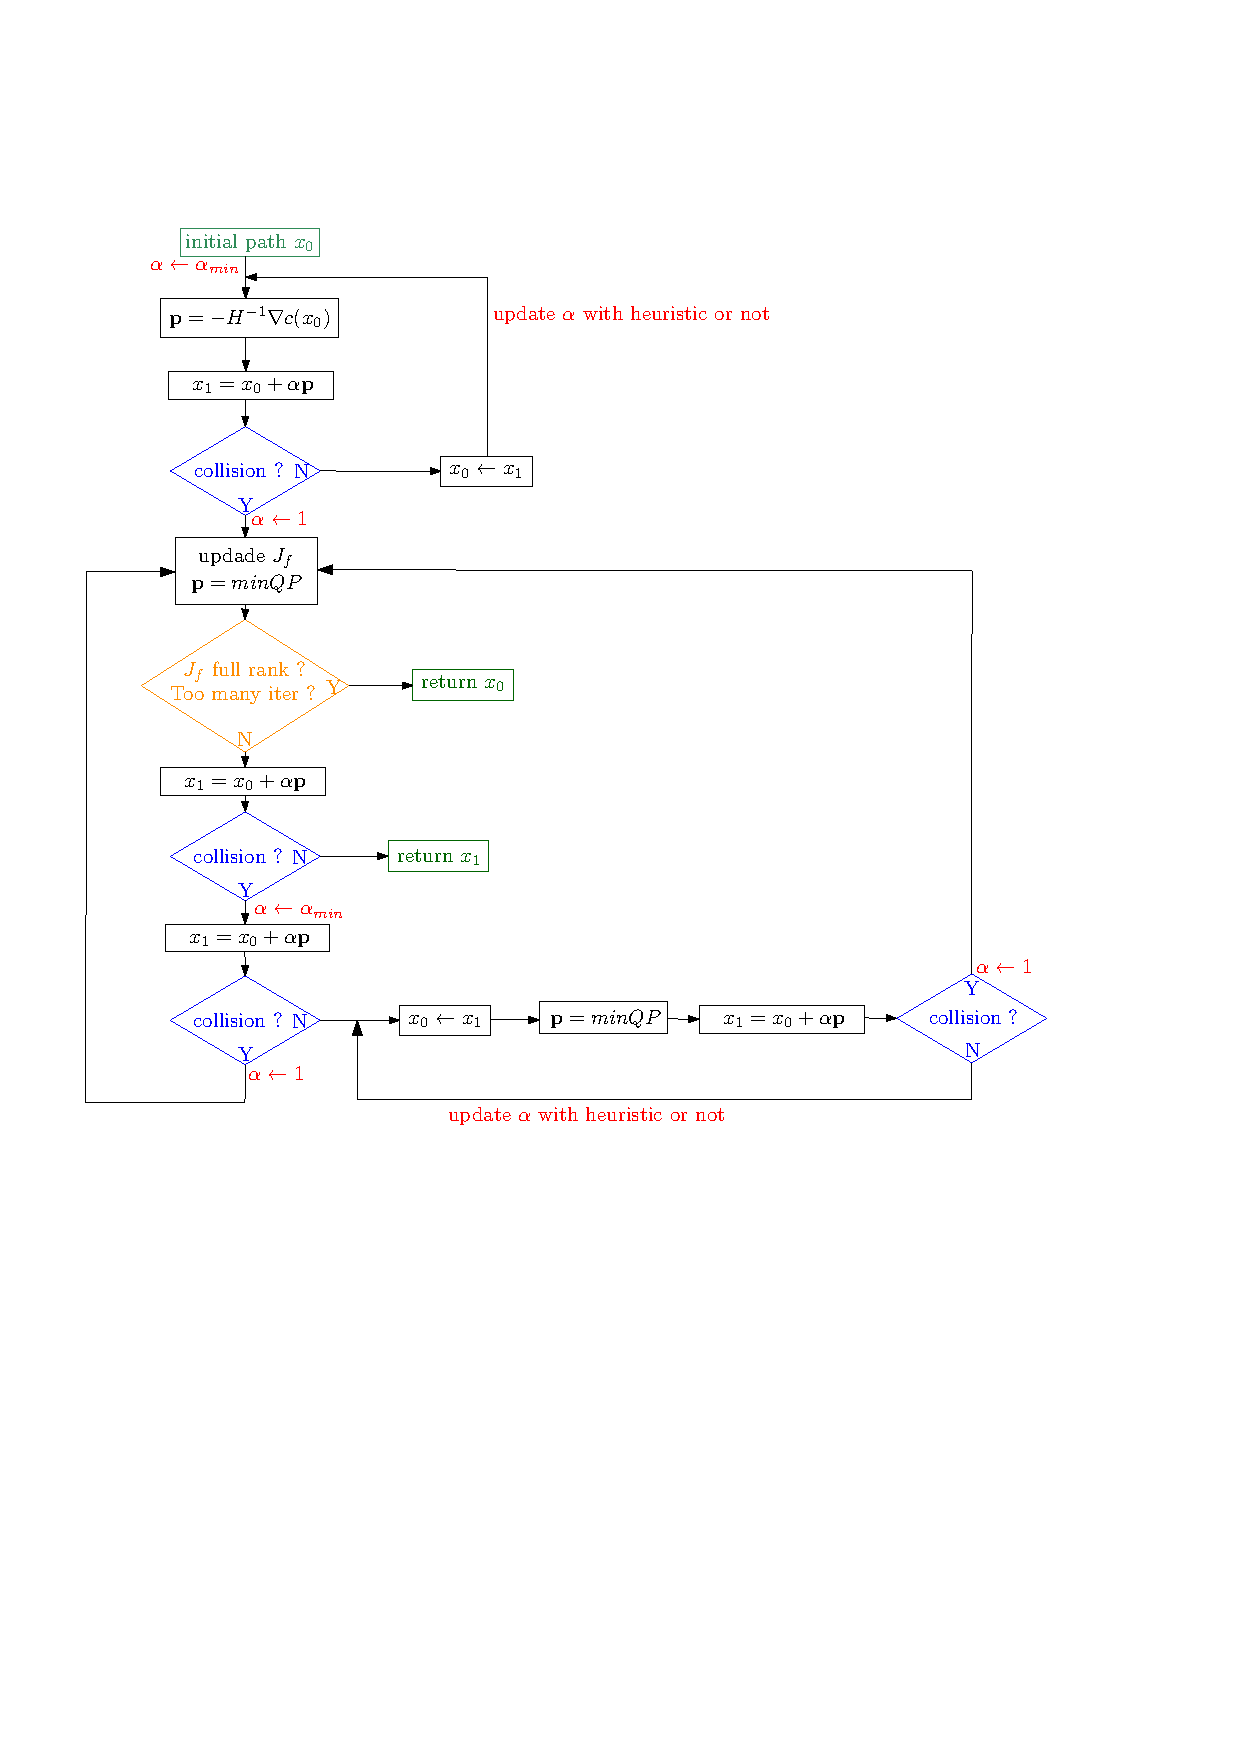
\includegraphics[width=14cm]{finiteStateMachine.pdf}
	\caption{Algorithm and alpha tuning. Number of algorithm iterations is 
increasing for each collision-test box. When reaching the command 
``update $Jf$'', collision information are gathered and constraints are 
computed, next paths will apply these constraints.}
	\label{fig:finiteStateMachine}
\end{figure}

\newpage

%%%%%%%%%%%%%%%%%%%%%%%%%%%%%%%%%%%%%%%%%%%%%%%%%%%%%%%%%%%%%%%%%%%%%%%%%%%%
\section{Weighted Cost}
\subsection{New cost definition}
Notation of length in configuration space: $i$ is the path (or iteration) index, 
$k$ is the waypoint (or sub-path) index. $n$ is the number of waypoints.
$$
L_{k,i} = || q_{k+1,i} - q_{k,i} ||
$$

Previously, we used the following quadratic cost:
$$
c(x_i) = \frac{1}{2}\sum_{k=0}^n {L_{k,i}^2}
$$

\textbf{Problem}: reducing this cost is reducing the length of the path BUT also
equidistantly allocating the waypoints. This represents a problem for long 
trajectories with local very-constrained paths as the puzzle and the 2D path
passing through a box.

\vspace{0.5cm}

\begin{wrapfigure}{r}{5cm}
	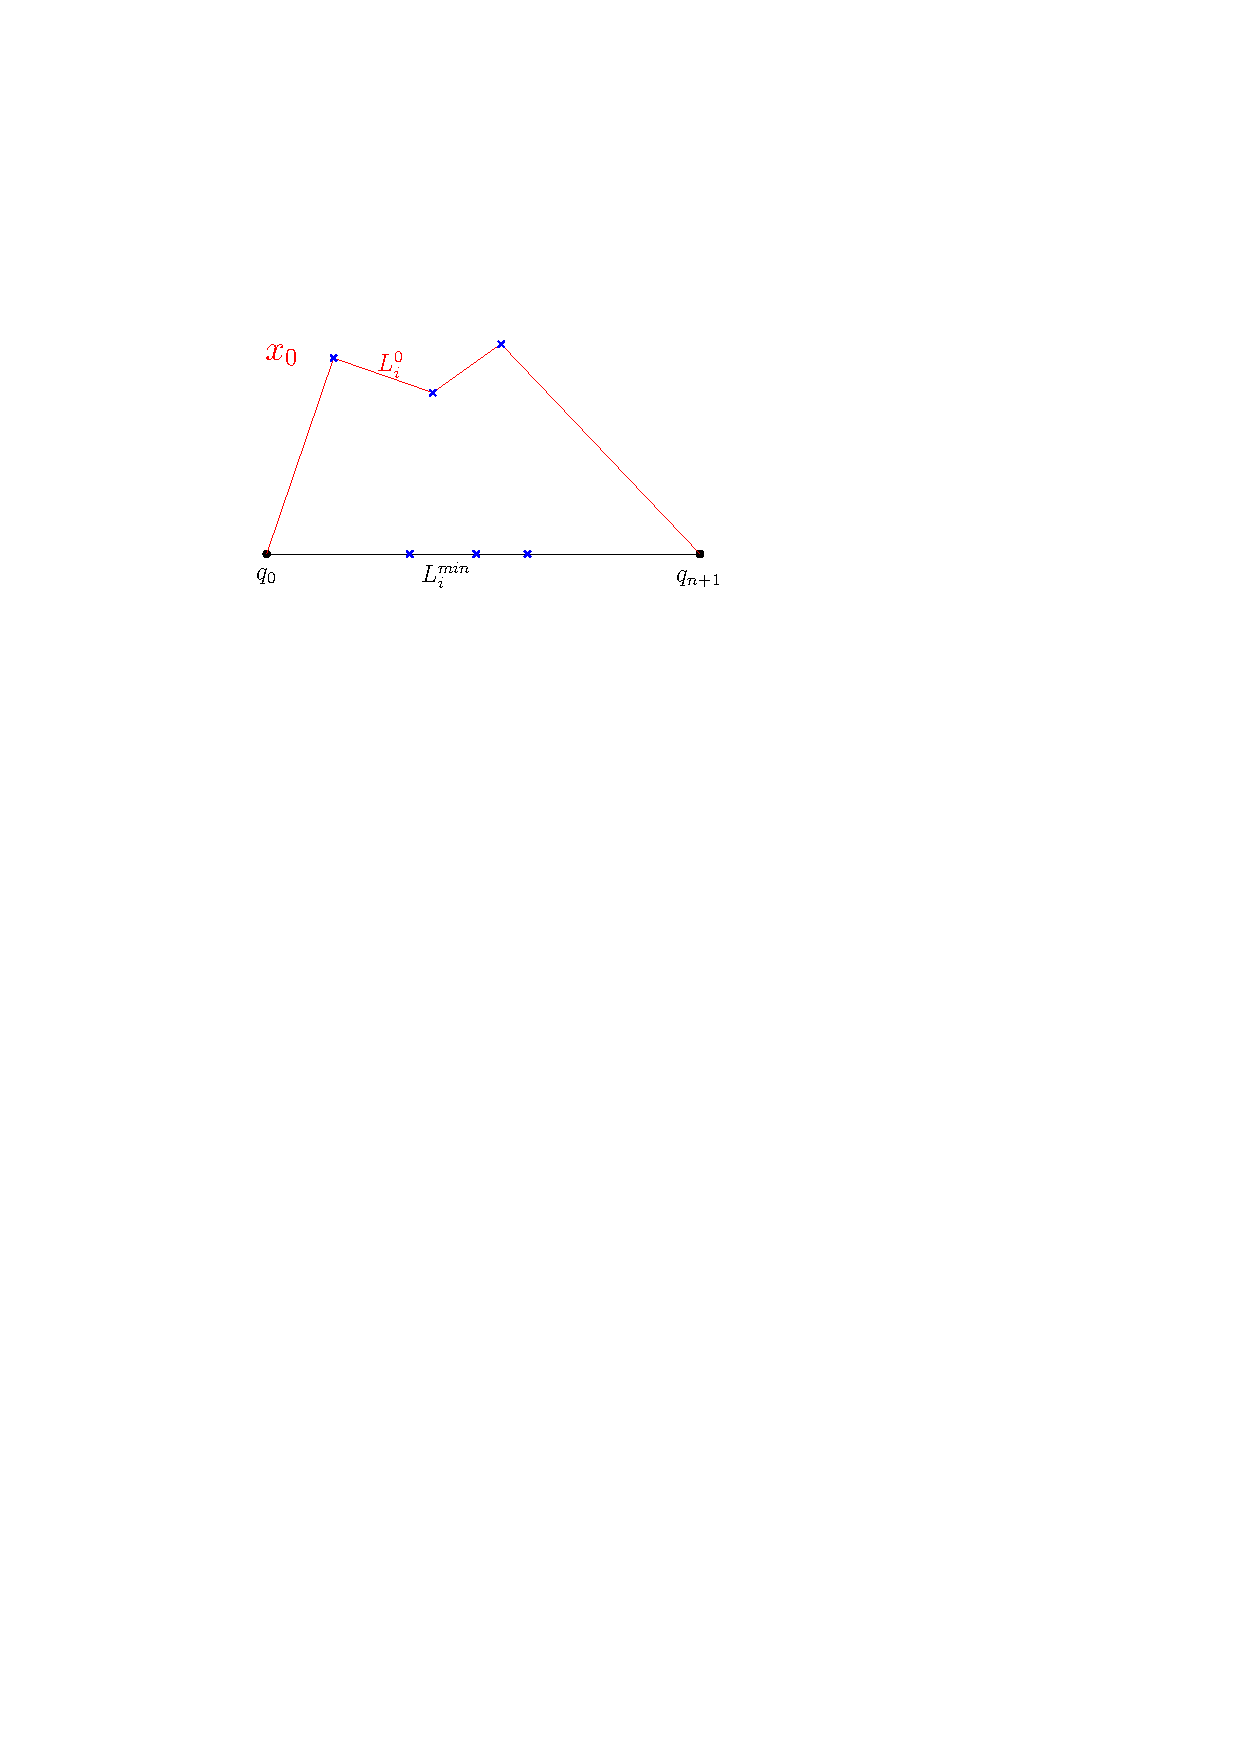
\includegraphics[width=5cm]{weighted_path.pdf}
	\caption{Illustration of an optimized path obtained by weighted cost. Note the 
	conservation of lengths proportionalites.}
	\label{fig:weightedCost}
\end{wrapfigure}

Therefore, we can use a weighted cost, according to the initial segments lengths :
$$
\forall k \in [0,n], \ \ w_k = \frac{1}{L_{k,0}}
$$
$$
c(x_i) = \frac{1}{2}\sum_{k=0}^n w_k{L_{k,i}^2}
$$

This cost has to propriety to conservate the proportionality (Fig. \ref{fig:weightedCost}) between of 
each segment length over total length between initial path $x_0$ and the ideal path 
without obstacle (so when the weighted gradient is zero) $x_{min}$.\\
The proportionality can be written as:
$$
\forall k \in [0,n], \ \ L_{k,min} = \frac{L_{min}}{L_{0}}L_{k,0}
$$

\vspace{0.4cm}

\subsection{Gradient implementation}

Lets $k\in [0;n]$ represents the waypoints index including initial and final 
configurations. Implemented previously:

\begin{wrapfigure}[9]{r}{5cm}
	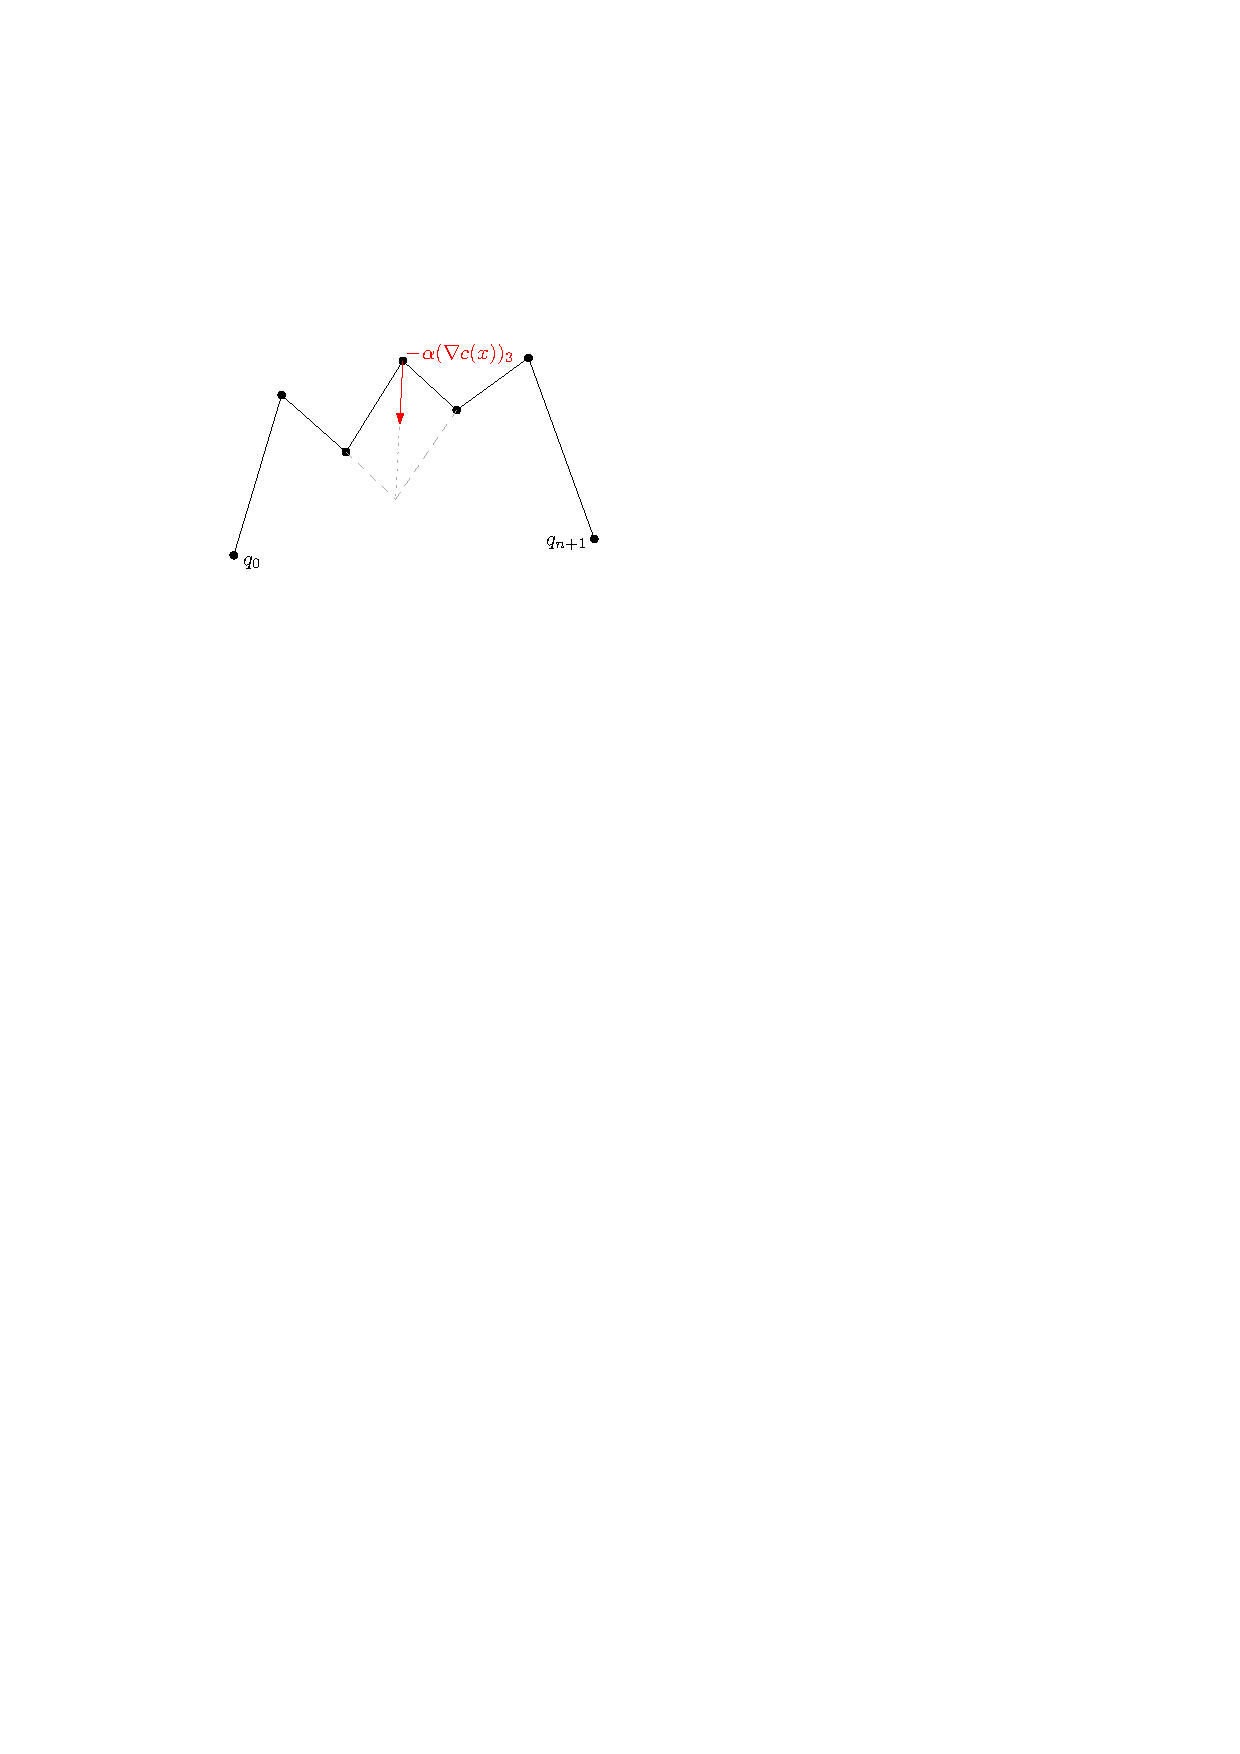
\includegraphics[width=5cm]{gradient.pdf}
	\caption{Illustration (without weights) of the third component of the path gradient.}
	\label{fig:gradient}
\end{wrapfigure}

$$
u1 = 
\left(\begin{array}{c} 
\vdots\\
q_{k+1} - q_k\\
\vdots
\end{array}
\right)^{k \in [0;n-1]}
$$
$$
u2 = 
\left(\begin{array}{c} 
\vdots\\
q_{k+2} - q_{k+1}\\
\vdots
\end{array}
\right)^{k \in [0;n-1]}
$$
$$
\nabla c(x) = u1 - u2 \ \in \real^n
$$

Now with weights (with the same notations):\\

$$
\nabla c(x) =
\left(\begin{array}{c}
w_0(q_{1} - q_{0}) -w_{1}(q_{2} - q_{1})\\
\vdots\\
w_{k-1}(q_{k} - q_{k-1}) -w_{k}(q_{k+1} - q_{k})\\
\vdots\\
w_{n-1}(q_{n} - q_{n-1}) -w_{n}(q_{n+1} - q_{n})\\
\end{array}
\right)^{k \in [1;n]}
$$

Note: for the ideal path where all points are aligned, the gradient is zero. 
Therefore:
$$
\forall k \in [1,n], \ \ w_{k-1}L_{k-1}^{min}  = w_{k}L_k^{min}
$$
$$
\forall k \in [1,n], \ \ w_{k-1}\frac{L^{min}}{L^{0}}L_{k-1}^{0}  = 
w_{k}\frac{L^{min}}{L^{0}}L_k^{0}
$$
And finally the equation that defines the cost weights:
$$
\forall k \in [1,n], \ \ w_{k-1}\,L_{k-1}^{0}  = w_{k}\,L_k^{0}
$$


\subsection{Hessian implementation}
$$
H(x) = \frac{\partial (\nabla c(x))}{\partial q}
$$
In practice:
\begin{align}
  \frac{\partial term_i}{\partial q_j}
  \begin{cases}
    w_{i-1}+w_i & \text{if }j=i\\
    -w_i  & \text{if }j=i+1\\
    -w_{i+1} & \text{if }j=i-1\\
  \end{cases}
\end{align}


So finally:
$$
H(x) =
\left(\begin{array}{ccccc}
(w_0+w_1)W & -w_1\,W & 0 & & \\
-w_1\,W & (w_1+w_2)W & -w_2\,W & 0 & \\
0 & -w_2W & (w_2+w_3)W & -w_3\,W & 0 \\
 &  &  & \ddots &  \\
 &  & 0 & -w_{n-1}\,W & (w_{n-1}+w_n)W \\
\end{array}
\right)
$$

Where $W$ is a diagonal matrix made of the robot weights.


\subsection{Example of results in 2D}

\begin{table}[h]
\centering
\begin{tabular}{cc}
	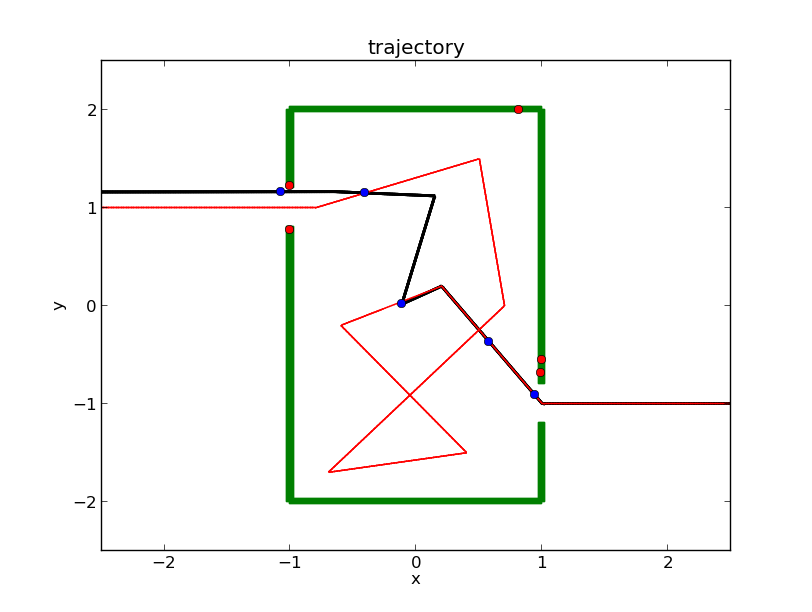
\includegraphics[width=6cm]{WEIGHTED_long_box100.png} &
	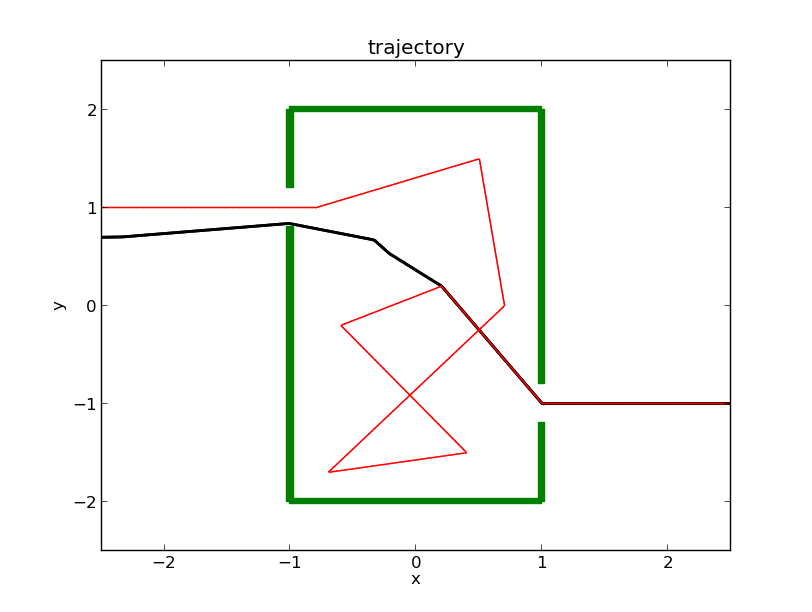
\includegraphics[width=6cm]{WEIGHTED_long_box100_2x.png}
\end{tabular}
	\caption{Result for a very long path from $(-100;1)$ to $(100;-1)$ which 
	Random Shortcut fails to optimize. Left: for $i_{max} = 30$ iterations 
	(local min obtained for 41 iterations exactly). Right: for $i_{max} = 30$ 
	iterations + second run of 14 iterations based on the first result. So we see 
	the interest of relaxing/canceling old constraints...}
\end{table}

\vspace{0.4cm}

%%%%%%%%%%%%%%%%%%%%%%%%%%%%%%%%%%%%%%%%%%%%%%%%%%%%%%%%%%%%%%%%%%%%%%%%%%%%
\newpage
\section{Work in progress}

\subsection{Affine constraints to compensate linearization error}

\begin{wrapfigure}[9]{r}{6cm}
	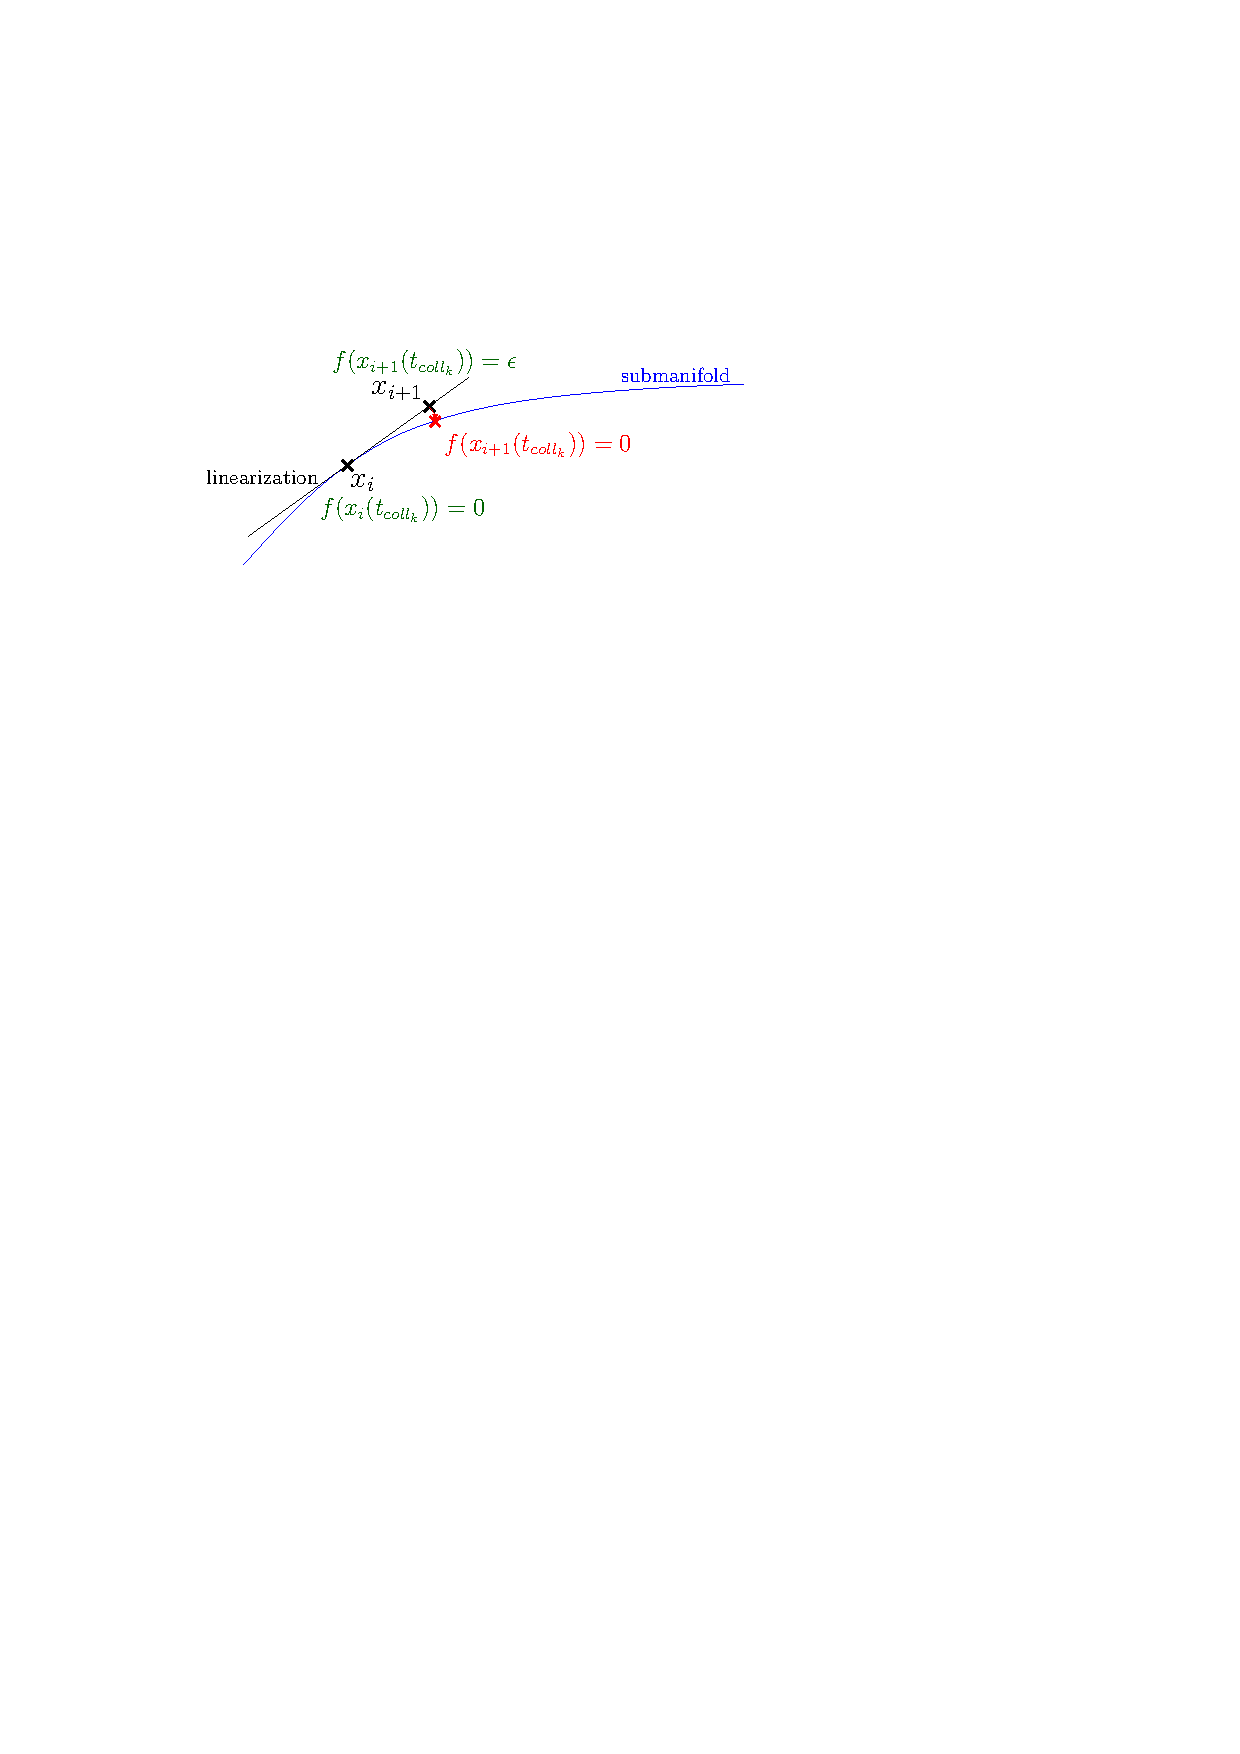
\includegraphics[width=6cm]{linearError.pdf}
	\caption{Linearization error.}
	\label{fig:linearError}
\end{wrapfigure}

In fact, for most of problems, the constraint function $f(q)$ is not linear. So during linearization on  $f$ constraint submanifold to compute the constraint jacobian $J_f$ a residual mistake may be encountered during the next iteration, if we re-check if the previous constraint is well-applied (Fig. \ref{fig:linearError}). We can also write this error as:
$$
f(x_0(\tcollk)) = 0 \ \ \text{path on which constraints are computed}
$$
$$
f(x_1(\tcollk)) = \epsilon \ \ \text{path on which constraints are applied}
$$
with $\tcollk$ the instant when collision occurs in the $k^{th}$ segment of the path.

\vspace{0.2cm}

But this approximation can be tolerated if there is no risk of collision. This criterion is 
obtained comparing the minimal distance $\mathscr{L}_d$ between the bodies that have been in collision at configuration $x_1(\tcollk)$ 
to the local range $\mathscr{R}$ of the constraint application error (similar to continuous collision checking):
$$
f(x_1(\tcollk)) = 
\begin{pmatrix}
t(M^{-1}\, M^*) \\
log(R^T\,R^*)
\end{pmatrix}
$$
$$
\mathscr{R} = r \, ||f(x_1(\tcollk))\,[3:6]|| + ||f(x_1(\tcollk))\,[0:3]||
$$
where $r$ is the \texttt{radius} of the joint, determined from the Device (see Fig. \ref{fig:framesConstraintError} for notations).

\begin{figure}[h]
	\centering
	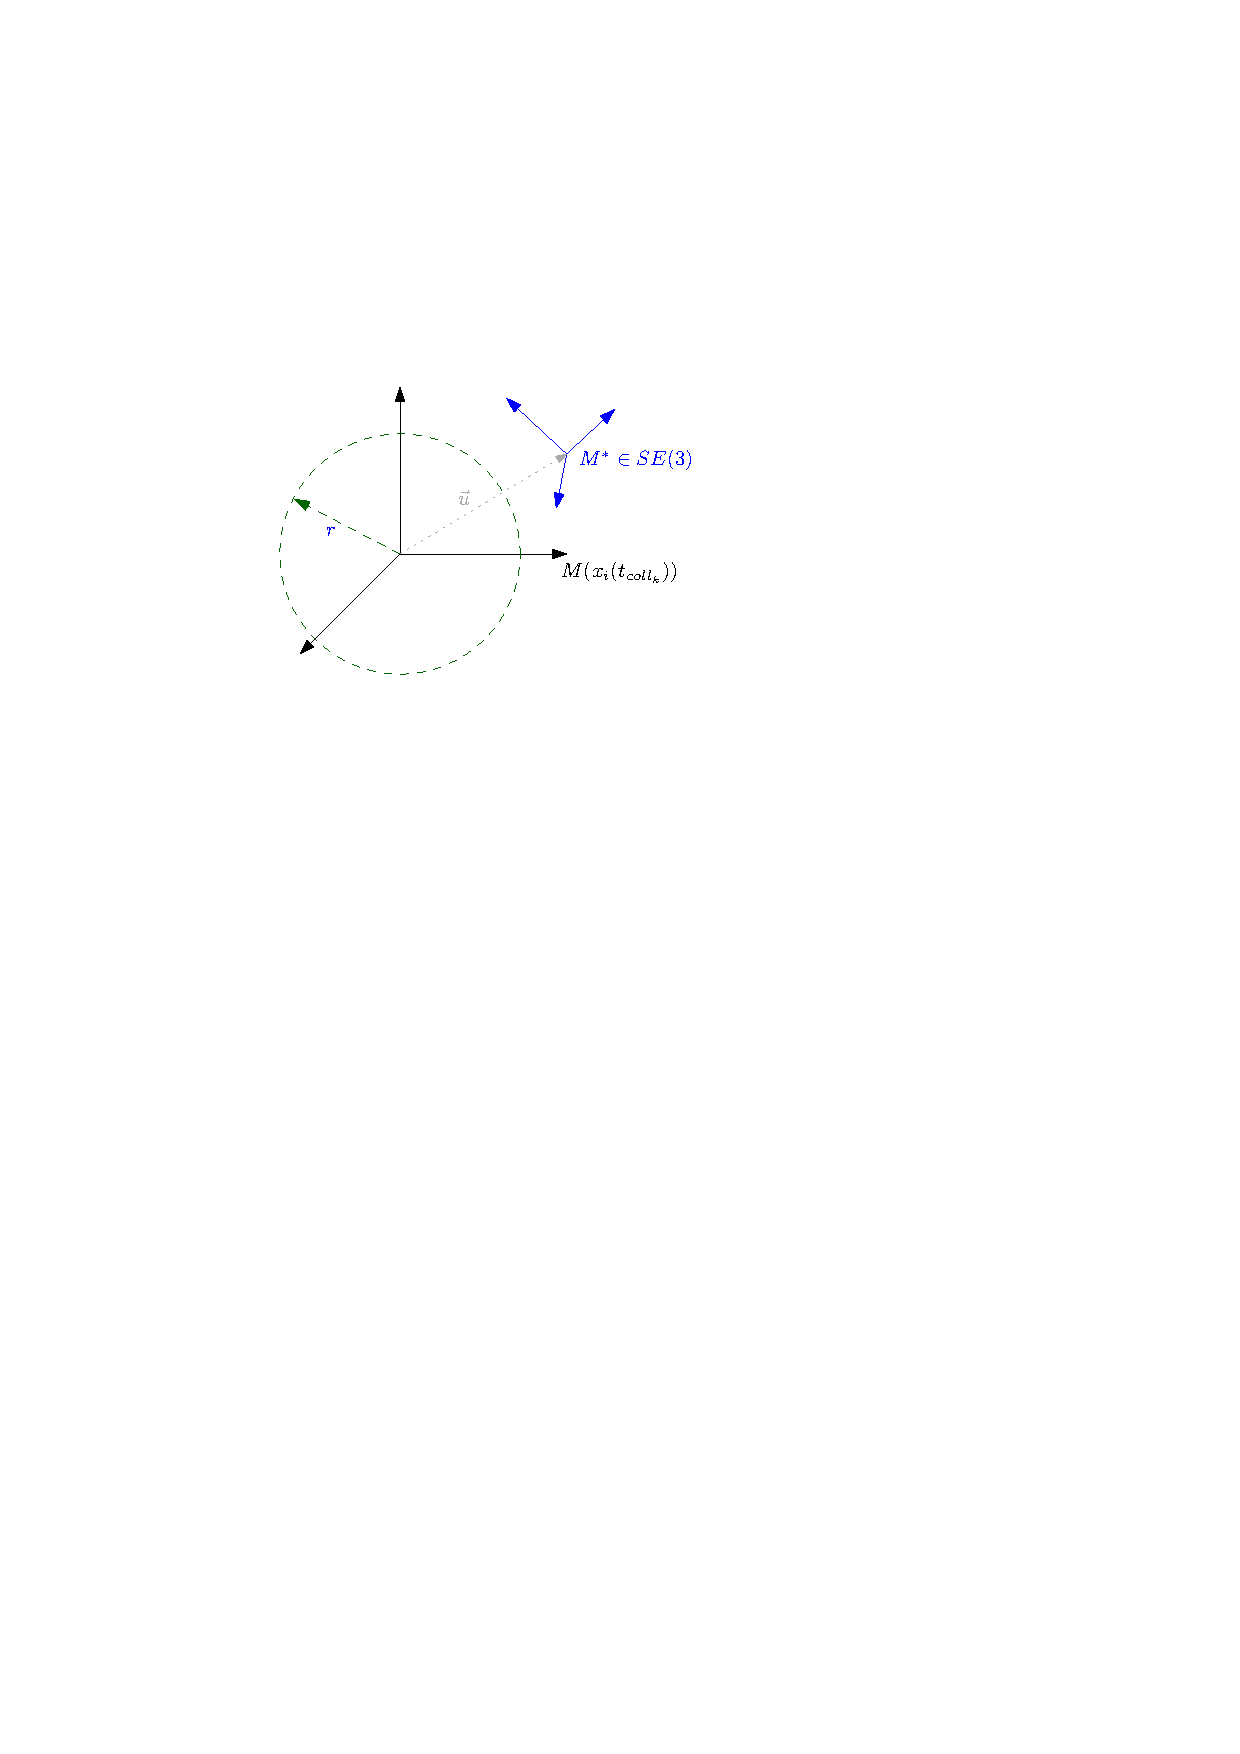
\includegraphics[width=6cm]{framesConstraintError.pdf}
	\caption{Collision-constraints frames notations.}
	\label{fig:framesConstraintError}
\end{figure}

\vspace{0.2cm}

Given a constraint $f$ linearized around $x_i$:
$$ f(x) = f(x_i) + J_f(x_i)\,(x_i) + o(x-x_i) \ \ \ \myeq  \ \ \ 0 $$
which gives (since $f(x_i)=0$):
$$ J_f(x_i)\,(x-x_i) \ \ \ \myeq  \ \ \ 0 $$
So we find our previous approach $ J_f\,\p = 0$.

\vspace{0.2cm}

In case we want to re-linearize this constraint around an other path $x_j$:
$$ f(x) = f(x_j) + J_f(x_j)\,(x_j) + o(x-x_j) \ \ \ \myeq  \ \ \ 0 $$
which gives
$$ J_f(x_j)\,(x-x_j) \ \ \ \myeq  \ \ \ -f(x_j) $$
So to re-linearize our constraint, we have to re-compute the constraint Jacobian on $x_j$ and to introduce and affine term $-f(x_j)$.


\vspace{0.2cm}

The following algorithm presents what is implemented as linear-error-compensation in the path-optimizer. As soon as a collision-constraint exists,\textsc{Compensation} is called after integrating the step and before testing path for collisions.

\begin{algorithm}
\caption{Raw version to summarize implemented work}
\label{algo:affineCompensation}
\begin{algorithmic}[1] % pour la numérotation des lignes
\Procedure{Compensation}{}
   \State a $m^{th}$ constraint exists at subpath rank $k$ and $t{_{coll_{k,m}}}$ parameter
   \State $x_i$ is collision-free
   \State $x_{i+1} \gets x_i + \alpha \p$
   \State $linErrorActive \gets False$
   \For{$m \in collisionConstraintsNumber$}
   		\State $q_{collConstr_m} \gets x_{i+1}(t{_{coll_{k,m}}})$
   		\State $\mathscr{R} \gets r \, ||f(q_{collConstr_m})\,[3:6]|| + ||f(q_{collConstr_m})\,[0:3]||$
   		\State $\mathscr{L}_d \gets \text{minDistance}(objects, q_{collConstr_m})$
   		\If{$\mathscr{R} > \mathscr{L}_d \ \mathbf{and} \ alpha != 1 $}
   			\State $linErrorActive \gets True$
   			\State A risk of collision due to linearization error exists !
   			\State Re-linearize $f_m$ around $q_{collConstr_m}$
   			% Strange since THIS config may be false due to the error
   			\State $J_{f_m}(x_{i+1})(x_{i+1}) = -f_m(x_{i+1})$
   			\State Replace $J_{f_m}$ in $J_f$ and $f_m$ in $b$
   		\EndIf
   \EndFor
   \If{$linErrorActive \textbf{ and }isValid(x1)$}
   		\State $\text{svd}(J_f,b)$ 
   		\State ($J_f$ is further used to compute $\mathbf{p}$)
   		\State $addConstraints \gets False$
   \EndIf
\EndProcedure
\end{algorithmic}
\end{algorithm}

Notes about the algorithm:
\begin{itemize}
\item (cf. test line 10): if $x_{i+1}$ (applying collision constraints) is computed 
with $\alpha=1$ and is not collision free, we choose to not waste time re-linearizing
 using $x_{i+1}$, because this path is `far' from the path that will be computed on the next step with $\alpha_{init}$ (when the $minQP$ is not collision-free, otherwise 
 the algorithm would be over whenever a need of compensation would have occured).
 
\item (cf line 20): it is difficult to modify $J_f$ at the same time with 
collision constraints and with re-linearisation. So whenever $x_{i+1}$ is in 
collision, and as soon as it was not computed with $\alpha=1$, linear compensation can 
be applicated \textbf{and} we will ignore $x_{i+1}$'s collision (because they could be caused by the linearization error itself!).

[Possible improvement] Test if the part $k$ of the path which is in collision is the same as the part on which compensation(s) occur(s). If not, we can re-linearize and add a new collision-constraint during the same path-iteration.

\item $addConstraint$ is a boolean tested when a collision is found on $x_{i+1}$ 
to determine if the associated constraint can be added. In the global algorithm 
figure \ref{fig:finiteStateMachine}, we can notice that $\alpha=1$ is also preventing from adding a new collision-constraint.
\end{itemize}


\vspace{0.2cm}




\newpage

%%%%%%%%%%%%%%%%%%%%%%%%%%%%%%%%%%%%%%%%%%%%%%%%%%%%%%%%%%%%%%%%%%%%%%%%%%%%
\section{Possible future work}

\subsection{Constraints relaxation}
In this part, some ideas for relaxing constraints are proposed.\\
In the case constraints are not directly canceled, but a compromise is found:
\begin{itemize}
\item Allow moving waypoints `connected' to some constraints to \textit{move} into the 
constraint direction ?
\item Add waypoints near a constraint to improve path-mobility ?
\end{itemize}

\vspace{0.4cm}
In the case we allow to cancel `old' constraints First.
\begin{itemize}
\item Define iteration threshold $i_{reset}$ from which constraints will be
canceled, based on an event such as:

\begin{itemize}
\item when improvement is not efficient anymore (\texttt{norm(s)} $< \epsilon$), which constraints are been canceled ? All ?
\item when algo tries to add existing constraints: on same localPath (\texttt{colRank}), 
same objects are in collision (with similar $\tcollk$ ?) Accepting how many constr before 
saying `no it is too similar' ? In this case, delete the old similar constraints
\end{itemize}

\item Or when the optimum under constraints has been reached, can try once more clearing all constraints 
(as when we relaunch manually). $i_{max}$ becomes the new criterion: number of tries to optimize path before give up

\item Use distances between bodies (\texttt{get\_dist}) ? May not be relevant, `cf potential' 
example: an annoying constraint is added at the bottom, but near an obstacle; so if we use a criterion `not cancel a constraint \textbf{near} an obstacle', this constraint will not be removed...

\end{itemize}

A completeness study should be provided when choosing beteween these ideas.


\vspace{0.4cm}

\subsection{Add problem constraints}
Initially, the planner provides a path containing waypoints and constraints. 
(Between two constrained waypoints, the interpolation does not garantee the constraint 
application for the whole path)

Basic sketch work:
\begin{itemize}
\item Remove initial path constraints and test if collision free. Depending on the 
answer, we will have to optimize keeping the constraints with the path or not.
\item Applies a local linearisation of the PB constraints on all waypoints: filling 
diagonally the Jacobian constraints $J\_$ with other problem-constraints Jacobians $J_{PB}$.
$$
J\_ =
\left(\begin{array}{cccc}
J_{PB} & & &0\\
 & J_{PB} & \\
 &  & \ddots   \\
0& & & J_{PB} \\
\end{array}
\right)
$$
Collision constraints $J_f$ will be simply added \textit{under} this matrix
$
\begin{pmatrix}
J\_ \\
J_f 
\end{pmatrix}
$

$\rightarrow$ \texttt{implemented in `GradientBased::getProblemConstraints'}

\item Project obtained path (waypoints) on PB constraints tangent space to correct 
waypoints (\texttt{ConfigProjector->projectOnKernel ()}). And then compute collisions...
\item If the PB constraints have been removed from the path in the first step, add 
them, project and test path. If in collision, stuck.
\end{itemize}



\vspace{0.4cm}

\subsection{Optimization on $SO(3)$ Lie group}

\begin{figure}[!h]
	\centering
	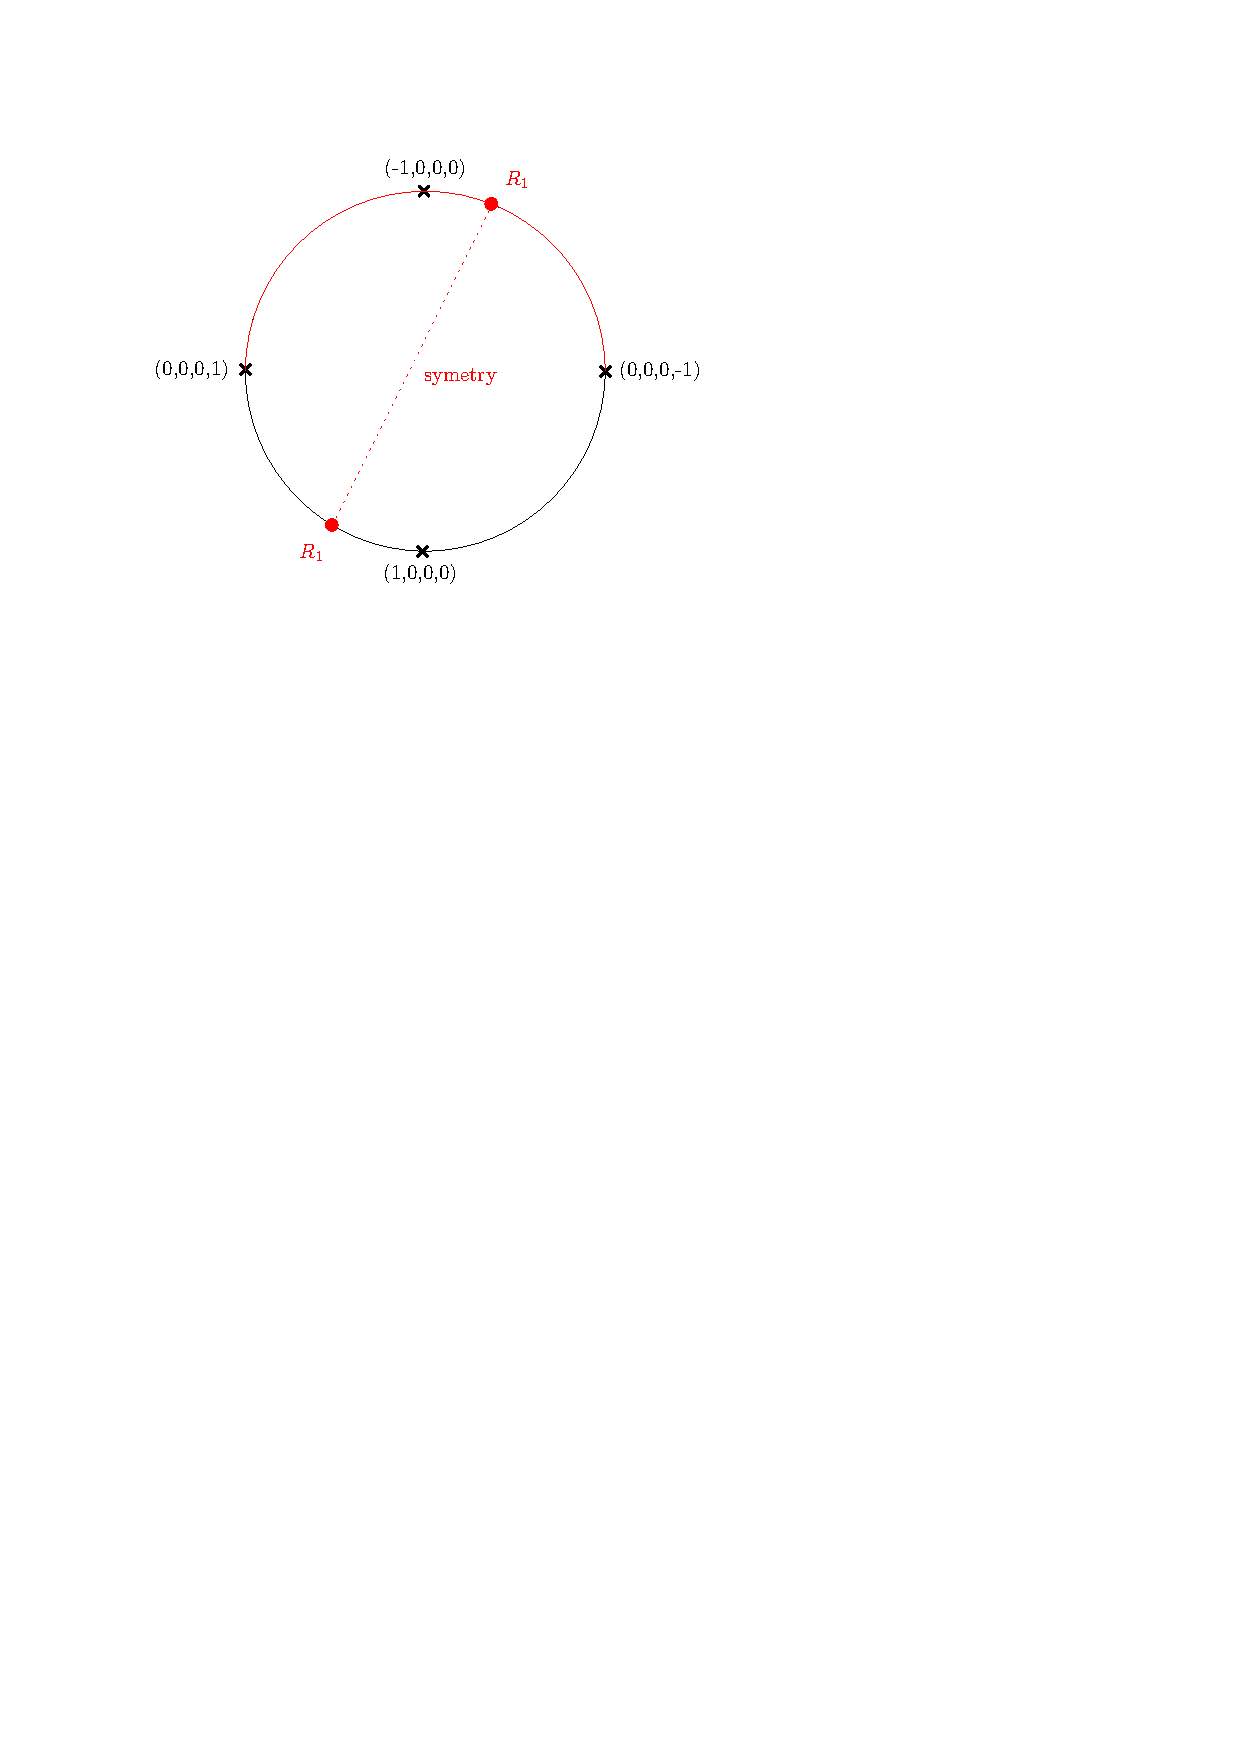
\includegraphics[width=6cm]{quaternions.pdf}
	\caption{Representation of a subpart of $SO(3)$ when only $\omega_z$ is 
	varying.}
	\label{fig:quaternions}
\end{figure}

QP resolution falling into local minimum of quaternion sphere (negative real part 
which corresponds to the same rotation).\\
See Fig. \ref{fig:quaternions}

Scalar product between $\mathbf{p}\nabla c(x)$ may be $<0$?

The gradient vanishes on a maximum (of length) instead a min?

\vspace{0.4cm}

\subsection{Waypoints prunning ?}
Kineo-like prunning method. Before calling optimizer ? But reduces optimization quality 
(less waypoints = less DoF for our problem, even if less time consuming)

\end {document}